\section{System Architecture}
\label{sec:system}

To describe our system, we first give an informal overview and then move on to the formal description.
Unlike most blockchain systems, we do not use a global ledger.
Instead, every node has their own hash chain.
The nodes only store transactions (TX) that they are involved in on their hash chain.
Transactions are stored in TX blocks and every block only contains one transaction.
We introduce a special block called checkpoint (CP) block, which represents the state of a hash chain.
Such data structure is called Extended TrustChain,
a visualisation can be seen on~\Cref{fig:trustchain-good-cp}.
\begin{figure}[h]
\centering
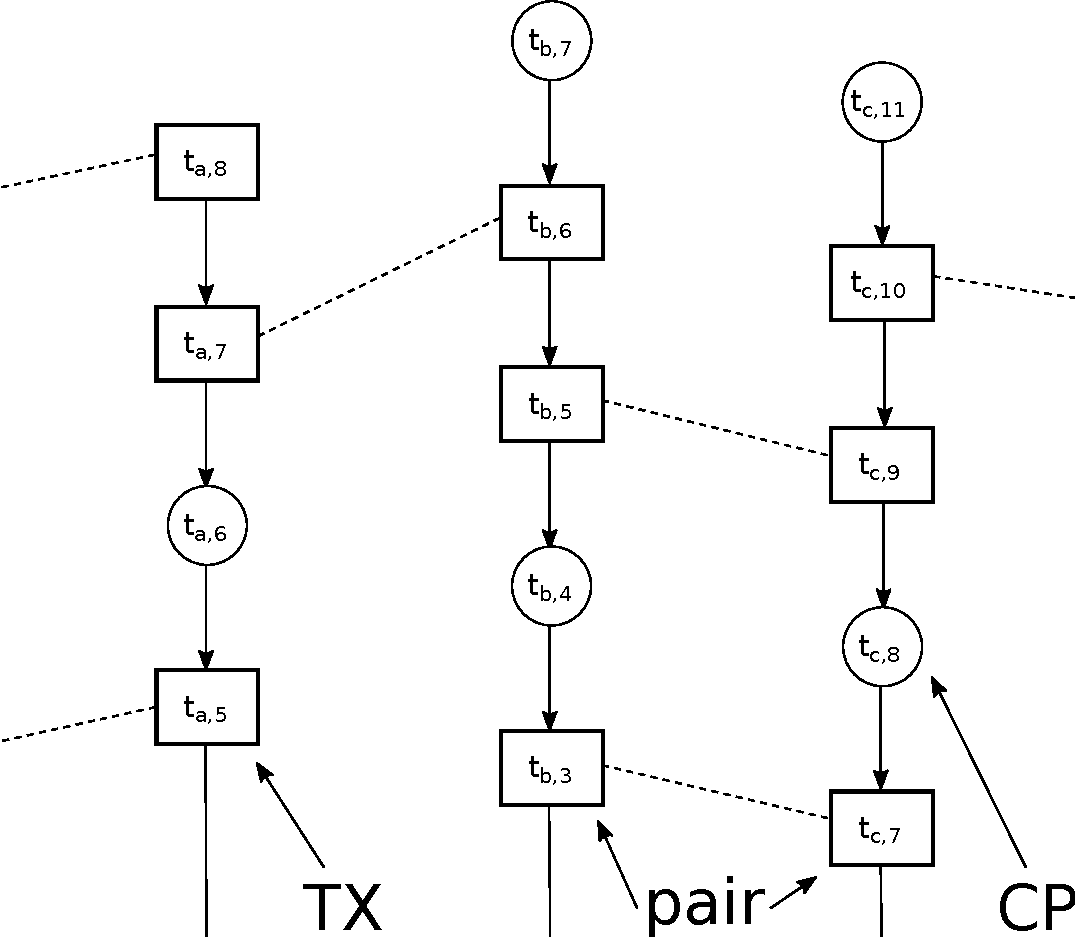
\includegraphics[width=\linewidth]{trustchain-good-cp}
\caption{Visualisation of the Extended TrustChain. $t_{u, i}$ represents a TX block on $u$'s chain with a sequence number of $i$.
$c_{v, j}$ represents a CP block on $v$'s chain with a sequence number of $j$.}
\label{fig:trustchain-good-cp}
\end{figure}

We randomly elect $n$ special nodes called facilitators in every round.
The facilitators reach consensus on CP blocks using an existing consensus algorithm---asynchronous subset consensus from HoneyBadgerBFT~\cite{miller2016honey}.
The consensus result is essentially a set of CP blocks from (nearly) all the nodes.
While this gives us consensus on a representation of the global state, it does not imply consensus on transactions.
To this end, we introduce a validation protocol that allows any nodes to challenge any other node to produce a set of TX blocks that computes to the CP block in consensus.
Hence we implicitly achieve consensus on transactions.
Since the transaction and validation protocols only make point-to-point communication,
we achieve horizontal scalability.

The formal description is given next,
it consist of one data structure---Extended TrustChain,
and three protocols---consensus protocol, transaction protocol and validation protocol.

\subsection{Extended TrustChain}
Each node $u$ has a public and private key pair---$pk_u$ and $sk_u$, and a chain $B_u$.
The chain consist of blocks $B_u = \{ b_{u, i} : i \in \{ 0, \dots, h - 1 \} \}$,
where $b_{u, i}$ is the $i$th block of $u$,
and $h$ is the height of the block (i.e. $h = |B_u|$).
We often use $b_{u, h}$ to denote the latest block.
There are two types of blocks, TX blocks and CP blocks.
If $T_u$ is the set of all TX blocks in $B_u$ and $C_u$ is the set of all CP blocks is $B_u$,
then it must be the case that $T_u \cup C_u = B_u$ and $T_u \cap C_u = \varnothing$.
The notation $b_{u, i}$ is generic over the block type.
We assume there exists a function $\textsf{typeof}: B_u \rightarrow \{ \tau, \gamma \}$ that returns the type of the block,
where $\tau$ represents the TX type and $\gamma$ represents the CP type.

\begin{definition}
\textbf{\emph{Transaction block}}

The TX block is a six-tuple, i.e
$$t_{u, i} = \langle \textsf{H}(b_{u, i - 1}), seq_u, txid, pk_v, m, sig_u \rangle.$$
We describe each item in turn.
\begin{enumerate}
\item $\textsf{H}(b_{u, i - 1})$ is the hash pointer to the previous block.
\item $seq_u$ is the sequence number which should equal $i$.
\item $txid$ is the transaction identifier, it should be generated using a cryptographically secure pseudo-random number generator by the initiator of the transaction.
\item $pk_v$ is the public key of the counterparty $v$.
\item $m$ is the transaction message.
\item $sig_u$ is the signature created using $sk_u$ on the concatenation of the binary representation of the five items above.
\end{enumerate}
The fact that we have no constraint on the content of $m$ is in alignment with our problem description---application neutrality.

TX blocks come in pairs.
In particular, for every block 
$$t_{u, i} = \langle \textsf{H}(b_{u, i - 1}), seq_u, txid, pk_v, m, sig_u \rangle$$
there exist one and only one \emph{pair} 
$$t_{v, j} = \langle \textsf{H}(b_{v, j - 1}), seq_v, txid, pk_u, m, sig_v \rangle.$$
Note that the $txid$ and $m$ are the same, and the public keys refer to each other.
Thus, given a TX block, these properties allow us to identify its pair.
\end{definition}

% TODO Node $v$ may cheat and create more than one pair for $t_{u, i}. we discuss later

\begin{definition}
\textbf{\emph{Checkpoint block}}

The CP block is a five-tuple, i.e. 
$$c_{u, i} = \langle \textsf{H}(b_{u, i-1}), seq_u, \textsf{H}(\C_r), r, sig_u \rangle,$$
where $\C_r$ is the consensus result (which we describe in \Cref{sec:consensus-result}) in round $r$,
the other items are the same as the TX block definition.
% Note that unlike in our prior work~\cite{implicitconsensus}, CP blocks and TX blocks do not have independent sequence numbers.

The genesis block in the chain must be a CP block in the form of
$$c_{u, 0} = \langle \textsf{H}(\bot), 0,  \textsf{H}(\bot), 0, sig_u \rangle,$$
where $\textsf{H}(\bot)$ can be interpreted as applying the hash function on an empty string.
The genesis block is unique because every node has a unique public and private key pair.
\end{definition}


\begin{definition}
\label{sec:consensus-result}
\textbf{\emph{Consensus result}}

Our consensus protocol runs in rounds.
Every round is identified by a round number $r$, which is incremented on every new round.
The consensus result is a tuple, i.e.
$$\C_r = \langle r, C \rangle,$$
where $C$ is a set of CP blocks agreed by the facilitators of round $r$.
\end{definition}

Here we define an important property which results from the interleaving nature of CP and TX blocks.
It is used in our validation protocol.
\begin{definition}
\textbf{\emph{Enclosure and agreed enclosure}}

If there exist a tuple $\langle c_{u,a}, c_{u, b} \rangle$ for a TX block $t_{u, i}$,
where 
$$a = \argmin_{k, k < i, \texttt{typeof}(b_{u,k}) = \gamma}(i - k)$$
$$b = \argmin_{k, k > i, \texttt{typeof}(b_{u,k}) = \gamma}(k - i),$$
then $\langle c_{u,a}, c_{u, b} \rangle$ is the enclosure of $t_{u, i}$.
Intuitively, that is the two closest CP blocks that surround $t_{u, i}$.
Note that $c_{u, a}$ is the more recent CP block.
Also, some TX blocks may not have any enclosure, then its enclosure is $\bot$.
Agreed enclosure is the same as enclosure with an extra constraint where the CP blocks must be in some consensus result $\C_r$.
\end{definition}


\begin{definition}
\textbf{\emph{Fragment and agreed fragment}}

If the enclosure of some TX block $t_{u, i}$ is $\langle c_{u,a}, c_{u, b} \rangle$,
then its \emph{fragment} $F_{u, i}$ is defined as $\{ b_{u, i} : a \le i \le b \}$.
Similarly, \emph{agreed fragment} has the same definition as fragment but using agreed enclosure.
For convenience, the function $\textsf{agreed\_fragment}(\cdot)$ represents the agreed fragment of some TX block if it exists, otherwise $\bot$.
\end{definition}

\subsection{Consensus Protocol}
Our scalable consensus protocol runs on top of Extended TrustChain.
It uses an unmodified asynchronous subset consensus (ACS) algorithm as the key building block (we describe the reasoning later).
The objectives of the protocol are to
allow honest nodes always make progress (in the form of creating new CP blocks),
compute correct consensus result in every round
and have an unbiased election of facilitators.
Concretely, we define the necessary properties as follows.
\begin{definition}
\label{def:consensus}
\textbf{\emph{Properties of the consensus protocol}}

$\forall r \in \mathbb{N}$, the following properties must hold.
\begin{enumerate}
    \item \emph{Agreement}:
        If one correct node outputs a set of facilitators $\F_r$,
        then every node outputs $\F_r$
    \item \emph{Validity}:
        If any correct node outputs $\F_r$, then 
            \begin{enumerate}
                \item $|\C_r| \ge N - t$ and each CP in $\C_r$ belong to a different node\footnote{
                $\C_r$ is a tuple but we abuse the notation here by writing $|\C_r|$ to mean the number of CP blocks in the second element of $\C_r$.}.
                \item $\F_r$ must contain at least $n - t$ honest nodes and
                \item $|\F_r| = n$.
            \end{enumerate}
    \item \emph{Termination}:
        Every correct node eventually outputs some $\F_r$.
    \item \emph{Fairness}:
        Every node with a CP block in $\C_r$ should have an equal probability of becoming a member of $\F_r$.
\end{enumerate}
\end{definition}
These properties are similar to Byzantine consensus properties but there are subtle differences.
Firstly, they are properties for every node in the network and not just the facilitators.
Secondly, they must be satisfied for all rounds,
because a failure in one round will lead to failures in sebsequent rounds.

\subsubsection{Bootstrap phase}
\label{sec:bootstrap}
As with many distributed systems, there must be a bootstrap phase which sets up the system.
Imagine that there is some bootstrap oracle, that initiates the code on every node.
The code satisfies all the properties in \Cref{def:consensus}.
Namely, every node has the same set of valid facilitators $\F_1$ that are randomly chosen.
This concludes the bootstrap phase.
For any future rounds, the consensus phase is used.

\subsubsection{Consensus phase}
\label{sec:consensus-phase}
The consensus phase begins when $\F_r$ is available to all the nodes.
Note that $\F_r$ indicates the facilitators that were elected using results of round $r$ and are responsible for driving the ACS protocol in round $r + 1$.
The goal is to reach agreement on a set of new facilitators $\F_{r + 1}$ that satisfies the four properties in \Cref{def:consensus}.

There are two scenarios in the consensus phase.
First, if node $u$ is not the facilitator, it sends $\langle \texttt{cp\_msg}, c_{u, h} \rangle$ to all the facilitators.
Second, if the node is a facilitator, it waits until $N - t$ messages of type \texttt{cp\_msg} are received.
% Second if the node is a facilitator, it waits for some duration $D$ and collect messages of type \texttt{cp\_msg}, where $D \gg \Delta$.
Invalid messages are removed.
That is blocks with invalid signatures and blocks signed by the same key.
With the sufficient number of \texttt{cp\_msg} messages,
it begins the ACS algorithm and some $\C'_{r + 1}$ should be agreed upon by the end of it.
Duplicates and blocks with invalid signatures are again removed from $\C'_{r+1}$ and we call the final result $\C_{r+1}$.
We have to remove invalid blocks a second time (after ACS) because the adversary may send different CP blocks to different facilitators,
which results in invalid blocks in the ACS output, but not in any of the inputs.

The core of the consensus phase is the ACS protocol,
it is based on the construction described in HoneyBadgerBFT~\cite{miller2016honey}.
We do not use the full HoneyBadgerBFT due to the following.
First, the transactions in HoneyBadgerBFT are first queued in a buffer and the main consensus algorithm starts only when the buffer reaches an optimal size.
We do not have an infinite stream of CP blocks, thus buffering is unsuitable.
Second, HoneyBadgerBFT uses threshold encryption to hide the content of the transactions.
But we do not reach consensus on transactions, only CP blocks, so hiding CP blocks is meaningless for us as it contains no transaction information.

Continuing, when $\F_{r}$ reaches agreement on $\C_{r+1}$,
they immediately broadcast\footnote{An alternative to using broadcasting is to use an epidemic protocl~\cite{eugster2004epidemic}, 
as long as it can guarantee delivery.} two messages to all the nodes---
first the consensus message $\langle \texttt{cons\_msg}, \C_{r+1} \rangle$,
and second the signature message $\langle \texttt{cons\_sig}, r, sig \rangle$.
The reason for sending \texttt{cons\_sig} is the following.
Recall that channels are not authenticated, 
and there are no signatures in $\C_{r + 1}$.
If a non-facilitator sees some $\C_{r + 1}$, it cannot immediately trust it because it may have been forged.
Thus, To guarantee authenticity, every facilitator sends an additional message that is the signature of $\C_{r + 1}$.

Upon receiving $\C_{r + 1}$ and at least $n - f$ valid signatures by some node $u$, $u$ performs two tasks.
First, it creates a new CP block using $\textsf{new\_cp}(\C_{r + 1}, r + 1)$ using \Cref{alg:new-cp}.
Second, it computes the new facilitators using $\textsf{get\_facilitator}(\C_{r + 1}, n)$ (\Cref{alg:facilitator}),
and updates its facilitator set to the result.
This concludes the consensus phase and brings us back to the state at the beginning of the consensus phase,
so a new round can be started.

\begin{algorithm}
\caption{Function $\textsf{new\_cp}(\C_r, r)$ runs in the context of the caller $u$.
It creates a new CP block and appends it to $u$'s chain.}
\label{alg:new-cp}
\begin{algorithmic}
\State $h \gets |B_u|$
\State $c_{u, h} \gets \langle \textsf{H}(b_{u, h-1}), h, \textsf{H}(\C_r), r, sig_u \rangle$
\State $B_u \gets B_u \cup c_{u, h}$
\end{algorithmic}
\end{algorithm}

\begin{algorithm}
\caption{Function $\textsf{get\_facilitator}(\C_r, n)$ takes the consensus result $\C_r$ and an integer $n$,
then sorts the CP blocks $C$ by the luck value (the $\lambda$-expression), and outputs the smallest $n$ elements.}
\label{alg:facilitator}
\begin{algorithmic}
\State $\langle r, C \rangle \gets \C_r$
\State $\textsf{take} (n, \textsf{sort\_by} (\lambda x.\textsf{H}(\C_r || pk \text{ of } x), C))$
\end{algorithmic}
\end{algorithm}


\subsection{Transaction Protocol}
\label{sec:tx-protocol}

The TX protocol, shown in \Cref{alg:tx-proto}, is run by all nodes.
It is also known as True Halves, first described informally by Veldhuisen~\cite[Chapter~3.2]{truehalves}.
Nodes that wish to initiate a transaction calls $\textsf{new\_tx}(pk_v, m, txid)$ (\Cref{alg:new-tx}) with the intended counterparty $v$ identified by $pk_v$ and message $m$.
$txid$ should be a uniformly distributed random value, i.e. $txid \in_R \{0, 1\}^{256}$,
then sends $\langle \texttt{tx\_req}, t_{u, h}\rangle$ to $v$.

\begin{algorithm}
    \caption{Function $\textsf{new\_tx}(pk_v, m, txid)$ generates a new TX block and appends it to the caller $u$'s chain.
    It is executed in the private context of $u$, i.e. it has access to the $sk_u$ and $B_u$.
    The necessary arguments are the public key of the counterparty $pk_v$, the transaction message $m$ and the transaction identifier $txid$.}
    \label{alg:new-tx}

    \begin{algorithmic}
    \State $h \gets |B_u|$
    \State $t_{u, h} \gets \langle \textsf{H}(b_{u, h - 1}), h, txid, pk_v, m, sig_u \rangle$
    \State $B_u \gets B_u \cup \{ t_{u, h} \}$
    \end{algorithmic}
\end{algorithm}

\begin{algorithm}
    \caption{The TX protocol which runs in the context of node $u$.}
    \label{alg:tx-proto}

    \begin{algorithmic}
        \Upon $\langle \texttt{tx\_req}, t_{v, j} \rangle$ from $v$
        \State $\langle \_, \_, txid, pk_v, m, \_ \rangle \gets t_{v, j}$
        \State $\textsf{new\_tx}(pk_u, m, txid)$
        \State store $t_{v, j}$ as the pair of $t_{u, h}$
        \State send $\langle \texttt{tx\_resp}, t_{u, h} \rangle$ to $v$

        \Upon $\langle \texttt{tx\_resp}, t_{v, j} \rangle$ from $v$
        \State $\langle \_, \_, txid, pk_v, m, \_ \rangle \gets t_{v, j}$
        \State store $t_{v, j}$ as the pair of the TX with identifier $txid$
    \end{algorithmic}
\end{algorithm}

A key feature of the TX protocol is that it is non-blocking.
At no time in \Cref{alg:new-tx} or \Cref{alg:tx-proto} do we need to hold the chain state and wait for some message to be delivered before committing a new block to the chain.
This allows for a high level of concurrency where we can call $\textsf{new\_tx}(\cdot)$ multiple times without waiting for the corresponding \texttt{tx\_resp} messages.

\subsection{Validation protocol}
\label{sec:vd-protocol}

Up to this point, we do not provide a mechanism to detect tampering.
The validation protocol aims to solve this issue.
The protocol is also a request-response protocol, just like the transaction protocol.
But before explaining the protocol itself, we first define what it means for a transaction to be valid.

\subsubsection{Validity definition}
A transaction can be in one of three states in terms of validity---\emph{valid}, \emph{invalid} and \emph{unknown}.
Given a fragment $F_{v, j}$,
the validity of the TX block $t_{u, i}$ with its corresponding fragment $F_{u, i}$ is captured by the function $\textsf{get\_validity}(t_{u, i}, F_{u, i}, F_{v, j})$ (\Cref{alg:get-validity}).
Note that $t_{u, i}$ and $F_{u, i}$ are assumed to be valid,
otherwise the node calling the function would have no point of reference.
This is not difficult to achieve,
because typically the caller is $u$, so it knows its own TX block and the corresponding agreed fragment.
If the caller is not $u$, it can always query for the agreed fragment that contains the transaction of interest from $u$.

% \Cref{alg:get-validity} works as follows.
% Before~\Cref{line:valid-fragment},
% we essentially check whether the fragment is the one that the verifier needs.
% If it is not, then the verifier cannot make any decision and return \emph{unknown}.
% This is likely to be the case for new transactions because the result of $\textsf{agreed\_fragment}(\cdot)$ would be $\bot$.
% The next two conditions check for tampering or missing blocks, if any of these misconducts are detected, then the TX is invalid.

We stress that the \emph{unknown} state means that the verifier does not have enough information to continue with the validation protocol.
If enough information is available at a later time, then the verifier will output either \emph{valid} or \emph{invalid}.

Note that the validity is on a transaction (two TX blocks with the same $txid$), rather than on one TX block owned by a single party.
It is defined this way because the malicious sender may create new TX blocks in their own chain but never send \texttt{tx\_req} messages.
In that case, it may seem that the counterparty, who is honest, purposefully omitted TX blocks.
But in reality, it was the malicious sender who did not follow the protocol.
Thus, in such cases, the whole transaction identified by its $txid$ is marked as invalid.

\begin{algorithm}
\caption{Function $\textsf{get\_validity}(t_{u, i}, F_{u, i}, F_{v, j})$ validates the transaction represented by $t_{u, i}$.
We assume $F_{u, i}$ is always correct and contains $t_{u, i}$.
$F_{v, j}$ is the corresponding fragment received from $v$.}
\label{alg:get-validity}

\begin{algorithmic}

    \If{$F_{v, j}$ is not a fragment created in the same round as $F_{u, i}$}
        \State \Return \emph{unknown}
    \EndIf

    \label{line:valid-fragment}
    \State $\langle \_, \_, txid, pk_v, m, \_ \rangle \gets t_{u, i}$
    \If{number of blocks of $txid$ in $F_{v, j} \ne 1$}
        \State \Return \emph{invalid}
    \EndIf

    \State $t_{v, j} \gets $ the TX block with $txid$ in $F_{v, j}$
    \State $\langle \_, \_, txid', pk_u, m', \_ \rangle \gets t_{v, j}$ 

    % message tampering
    \If{$m \ne m' \vee txid \ne txid'$} 
        \State \Return \emph{invalid}
    \EndIf

    % signature tampering
    \If{$t_{u, i} \text{ is not signed by } pk_u \vee t_{v, j} \text{ is not signed by } pk_v $}
        \State \Return \emph{invalid}
    \EndIf
    \State \Return \emph{valid}
\end{algorithmic}
\end{algorithm}

\subsubsection{Validation protocol}
Our validation protocol,
shown in~\Cref{alg:vd-proto},
is designed to classify transactions according to the aforementioned validity definition.
If $u$ wishes to validate some TX with ID $txid$ and counterparty $v$, it sends $\langle \texttt{vd\_req}, txid \rangle$ to $v$.
The desired properties of the validation protocol are as follows.
\begin{definition}
\label{def:validation}
\textbf{\emph{Properties of the validation protocol}}

\begin{enumerate}
    \item \emph{Agreement}:
        If any correct node decides on the validity (except when it is \emph{unknown}) of a transaction,
        then all other correct nodes are able to reach the same conclusion or \emph{unknown}.
    \item \emph{Validity}:
        The validation protocol outputs the correct result
        according to the aforementioned validity definition.
    % \item \emph{Unforgeability}:
    %     If some transaction is valid, it cannot be forged into an invalid transaction.
    %     If some transaction is invalid, it cannot be forged into a valid transaction.
    \item \emph{Liveness}:
        Any valid (invalid) transaction is marked as valid (invalid) eventually.
\end{enumerate}
\end{definition}

\begin{algorithm}
\caption{Validation protocol which runs in the context of $u$}
\label{alg:vd-proto}

\begin{algorithmic}
    \Upon $\langle \texttt{vd\_req}, txid \rangle$ from $v$
        \State $t_{u, i} \gets \text{the transaction identified by } txid$
        \State $F_{u, i} \gets \textsf{agreed\_fragment}(t_{u, i})$
        \State send $\langle \texttt{vd\_resp}, txid, F_{u, i} \rangle$ to $v$

    \Upon $\langle \texttt{vd\_resp}, txid, F_{v, j} \rangle$ from $v$
        \State $t_{u, i} \gets \text{the transaction identified by } txid$
        \If{$F_{u, i}$ and $F_{v, j}$ are available and $F_{u, i}$ is the agreed fragment of $t_{u, i}$}
            \State set the validity of $t_{u, i}$ to $\textsf{get\_validity}(t_{u, i}, F_{u, j}, F_{v, j})$
        \EndIf
\end{algorithmic}
\end{algorithm}

We make two remarks.
First, just like the TX protocol, we do not block at any part of the protocol.
Second, suppose some $F_{v, j}$ validates $t_{u, i}$, then that does not imply that $t_{u, i}$ only has one pair $t_{v, j}$.
Our validity requirement only requires that there is only one $t_{v, j}$ in the correct consensus round.
The counterparty may create any number of fake pairs in later consensus rounds.
But these fake pairs only pollutes the chain of $v$ and can never be validated because the round is incorrect.

\subsection{Design variations and tradeoffs}
\label{sec:tradeoffs}
In this section, 
we explore a few design variations which we can make, some of them require a relaxed version of our original model.
They enable better performance and allow us to apply our design in the fully permissionless setting.

\subsubsection{Using timing assumption in the permissionless setting}
\label{sec:permissionless}
One limitation of our system is that we use the parameter $N$ in our algorithms, which makes it unsuitable for the permissionless environment where users can join and leave at will.
In this section we show how making a timing assumption would allow us to operate in the permissionless setting.

At the start of our consensus phase (\Cref{sec:consensus-phase}), facilitators must wait for $N-f$ \texttt{cp\_msg} messages.
This is the only place where we used $N$ as a parameter.
To introduce timing, instead of waiting for $N-f$ messages, we wait for some time $D$,
such that $D$ is sufficiently long for honest nodes to send their CP blocks to the facilitators.
Consequently, this removes the need for a PKI because the collected CP blocks may be from nodes that nobody has seen in the past.

The new protocol handles churn as follows.
Suppose a new node wish to join the network and the facilitators are known (this can be done with a public registry).
It simply sends its latest CP block to the facilitators.
Then, in the next round, the node will have a chance to become a facilitator just like any existing node.
To leave the network, nodes simply stop submitting CP blocks.
There is a subtlety here which happens when the node is elected as a facilitator in the following round.
In this case, the node must fulfil its obligation by completing the consensus protocol, but without proposing its own CP block, before leaving.
Otherwise, the $n \ge 3t + 1$ condition may be violated.

\subsubsection{Optimising validation protocol using cached agreed fragments}
\label{sec:caching}
One more way to improve the efficiency of the validation protocol is to use a single agreed fragment to validate multiple transactions.
Concretely, for node $A$, upon receiving an agreed fragment from node $B$,
rather than validating a single transaction,
$A$ attempts to validate all transactions with performed with $B$ in the unknown state, in that fragment.

The benefit of this technique is maximised when a node only transacts with one other node.
In this case, the communication of one fragment is sufficient to validate all transactions in that fragment.
In the opposite extreme, if every transaction that the node makes is with another unique node,
then the caching mechanism would have no effect.

\subsubsection{Total fork detection}
\label{sec:fork}
The validation algorithm guarantees that there are no forks within a single agreed fragment.
This is sufficient for some applications such as proving the existence of some information.
However, for applications such as digital cash where every block depends on one or more previous blocks,
our scheme is not suitable.
For such applications, we need to guarantee that there are no forks from the genesis block leading up to the TX block of interest.

We offer two approaches to do total fork detection.
First and the easiest solution is to simply ask for the complete chain of the counterparty.
The verifier can be sure that there are no forks if the following holds.
\begin{enumerate}
    \item The hash pointers are correct.
    \item All the CP blocks are in consensus.
    \item The TX of interest is in the chian.
\end{enumerate}
We use this approach in our prior work on Implicit Consensus~\cite{implicitconsensus}.
Nodes employ caching to minimise communication costs, we call this effect spontaneous sharding.

The second approach is probabilistic but with only a constant communication overhead over our current design.
For a node, observe that if all of its agreed fragments has a transaction with an honest node,
then the complete chain is effectively validated in a distributed manner.
The only way for an attacker to make a fork is to make sure that the agreed fragment containing the fork has no transactions with honest nodes.
Such malicious behaviour is prevented probabilistically using a challenge-response protocol as follows.
Suppose node $A$ wish to make a transaction with node $B$.
$A$ first sends a challenge to $B$ asking it to prove that it holds a valid agreed fragment between some consensus round specified by $A$.
If $B$ provides a correct proof, then they run the transaction protocol as usual.
If $B$ provides an invalid proof or refuses to respond,
then $A$ would refuse to make the transaction.

